\subsection{2.3.1. 跨层 KV 与索引复用}\label{cross-layer-kv-and-index-reuse}

每个 CSA2 层被静态分配三种模式之一：Full、
Reindex 或 Reuse。在全部三种模式下，该层都计算自己的 query
和 SWA KV，并将其与选定的主 KV 条目一起用于
产生新的注意力输出。各模式的区别在于如何获取主
KV、索引器 K 和 Top-K 索引。图 4 展示了这三种模式。

Full 模式。该层计算自己的主 KV 和索引器 Q，从主
KV 投影出索引器 K，并运行索引器以产生全新的 Top-K
索引。因此它执行完整的 CSA2 计算路径，其组件职责与
DeepSeek-V4 中完整的 CSA2 层








相同。

Reindex 模式。该层复用前面一层中最近可用的主 KV
以及与之对应的索引器 K。索引器计算自己的 query，
对复用的键重新评分，并产生全新的 Top-K
索引。这允许稀疏选择跨层发生变化，
而主 KV 和索引器 K 保持共享。

Reuse 模式。该层复用最近可用的主 KV 和最新
的 Top-K 索引，后者由处于 Full 或 Reindex 模式的前面层
针对该主 KV 计算得出。它使用这一选择执行注意力，
不计算索引器 Q，也不评估索引分数。

共享主 KV 和索引器 K 可减少缓存存储，而复用 Top-K
索引可避免额外的索引器计算。Reindex 模式在保持
缓存共享的同时，允许所选条目跨层发生变化。当
CSA2 与 CED 结合时，被分配为 Full 模式的解码器层会
从第 $(L/2)$ 层的隐藏状态计算自己的全局 KV，即因果编码器的最后一层。Reindex
和 Reuse 模式保持不变。

\subsection{2.3.2. 层次化稀疏索引器}\label{hierarchical-sparse-indexer}

跨层索引复用减少了索引器评估的次数，但
剩余索引器仍要对完整的因果可见上下文进行评分。
对于极长上下文，这一代价仍是主要的计算
瓶颈。此前的工作通过评分
和剪枝池化块表示，在 token 级索引之前引入了索引器
稀疏性（Xu et al., 2026b）。我们发现，在解码器中，较浅层
索引器的信息自然可以用来限制较深层索引器
所考虑的候选，而无需增加任何额外状态。因此我们引入了
层次化稀疏索引器，它仅用于 CED 的
解码器，以减少解码期间的这种重复评分。对于每个 query，
第一个被分配为 Full 模式的层构建一个候选池，后续
重新索引的各层将其用作搜索域。在候选池大小
固定时，较深层索引器的单 query 代价从关于上下文长度的线性
变为常数。该机制是训练感知的，并在后训练中引入：
候选限制在训练和推理期间以相同方式应用，
因此较深层索引器在与推理时相同的搜索域下被
优化。图 5
说明了这一过程。





第一个 Full 模式层对所有因果可见的主 KV 位置进行评分，
并为其自身注意力产生 Top-K 索引。它还进行
块级候选选择：每个块被赋予其各位置中最大的索引
分数，得分最高的块被选中。然后它将所选块覆盖的位置
收集到一个
比最终 Top-K 集合更大的候选池中。例如，
选择 2,048 个块，每块 8 个位置，可得到 16,384 个候选
位置。该池定义了后续索引器搜索的范围；最终的
Top-K 选择决定每一层读取哪些主 KV 条目。

处于 Reindex 模式的后续层仅对相应 query 的候选位置
进行评分，并在该池内选择自己的 Top-K 条目。处于 Reuse
模式的层不进行新的索引，直接使用针对所复用主 KV 计算出的
最新 Top-K 索引。因此，
候选池在索引层之间共享，而它们最终的
选择可以不同。

在候选池大小固定的情况下，每个后续索引器对每个
query 评分的位置数有界，与上下文
长度无关。第一个 Full 模式层仍会扫描整个因果可见
范围。因此，层次化索引在保留最初的全局扫描的前提下，
降低了后续索引器评估的代价。

\subsection{2.4. 高效的架构扩展}\label{efficient-architectural-extensions}

\subsection{2.4.1. 单遍 mHC}\label{single-pass-mhc}

在 DeepSeek-V4 中，我们引入了 mHC（Xie et al., 2026），它在相邻 Transformer
块之间维护 $n$ 条残差流。对每个 token，我们
用 \(X _ { l } \in \mathbb { R } ^ { n \times d }\)
表示这些流，其中 $l$ 是块索引，$d$ 是隐藏维度。这些流
按如下方式更新：

\[
X _ { l + 1 } = B _ { l } X _ { l } + C _ { l } { \mathcal { F } } _ { l } ( A _ { l } X _ { l } ) , \qquad ( A _ { l } , B _ { l } , C _ { l } ) = { \mathcal { H } } ( X _ { l } ) ,\tag{2}
\]

其中
\(A _ { l } \in \mathbb { R } ^ { 1 \times n } , C _ { l } \in \mathbb { R } ^ { n \times 1 }\)
且 \(B _ { l } \in \mathbb { R } ^ { n \times n }\) 是由 $X_l$ 预测的
token 级系数。系数预测器 H 包括
归一化和投影。

理想情况下，两个块之间的残差变换是一个从
\(\left( X _ { l - 1 } , Y _ { l - 1 } \right)\) 到
\(( X _ { l } , \hat { X } _ { l } )\) 的单一映射，其中
\(\hat { X } _ { l } = A _ { l } X _ { l }\) 是当前块的输入，
而
\(Y _ { l - 1 } = \mathcal { F } _ { l - 1 } ( \hat { X } _ { l - 1 } )\)
是上一块的输出。这样的映射需要 $(n + 1)d$ 次读取和
\(( n + 1 ) d\) 次写入，从而对激活内存访问量给出
\(( 2 n + 2 ) d\) 的下界。实际上，DeepSeek-V4 采用公式 (2) 的多遍
实现，包含三个因数据依赖而顺序执行的
内核：

\[
X _ { l } = B _ { l - 1 } X _ { l - 1 } + C _ { l - 1 } Y _ { l - 1 } \qquad { \mathrm { R e s i d u a l ~ u p d a t e , c o n t r a c t i o n ~ o v e r ~ } } n\tag{3}
\]

\[
\left( A _ { l } , B _ { l } , C _ { l } \right) = \mathcal { H } ( X _ { l } )
\]

\[
\mathbf { C o e f f i c i e n t s , c o n t r a c t i o n o v e r } n d\tag{4}
\]

\[
\hat { X } _ { l } = A _ { l } X _ { l }
\]

\[
{ \mathrm { I n p u t m i x i n g } } , { \mathrm { c o n t r a c t i o n o v e r } } n\tag{5}
\]

这三个内核分别读取 $((n + 1)d$、$nd$ 和 $nd$ 个值，
总共写入 \(( n + 1 ) d\)。把
\(\mathcal { F } _ { l } ,\) 中的预归一化算在内，总的激活内存访问量为
\(( 4 n + 4 ) d ,\) , 是下界的两倍。

在 H 中，归一化权重被离线折叠进投影权重，
RMS 除法在投影之后应用。三个阶段中有两个
因此可以共享对残差的一次遍历：
残差更新不需要跨隐藏维度做归约，
因此 \(X _ { l }\) 的每个 tile 都可以被计算出来并立即
用于累加计算 RMS 所需的投影输出和平方和。
输入混合无法融合进这一遍，因为
在对所有隐藏 tile 完成归约之前，
\(A _ { l }\) 不可用。因此它需要对 \(X _ { l } .\) . 进行第二次读取。
这第二遍还可以并入输入预归一化。这种两遍
实现总共需要 $(3n + 2)d$ 次激活读取和写入，
与下界
相比，多了一次对 \(X _ { l }\) 的读取。




因此，我们引入了单遍 mHC：它将输入混合
系数错移一个块，即每个块使用前一个块产生的混合
系数，从而使上述依赖
消失：

\[
X _ { l + 1 } = B _ { l } X _ { l } + C _ { l } \mathcal { F } _ { l } ( A _ { l - 1 } X _ { l } ) , \qquad ( A _ { l } , B _ { l } , C _ { l } ) = \mathcal { H } ( X _ { l } ) .\tag{6}
\]

输入混合现在使用 \(A _ { l - 1 }\) 而不是 \(A _ { l } ,\)，因此它
不再依赖根据 \(X _ { l } .\) . 计算出的系数。
因此，$X_l$ 的每个 tile 可以立即同时用于输入混合
和系数预测，而无须等待完整的归约。
经验上，这种错移带来的性能退化可以忽略不计。

对于预训练，我们保留现有的多内核实现，
因为这种错移只是改变了每个块所应用的混合系数。
对于部署，我们将残差更新、输入混合和
系数预测融合为单一内核 Mega-mHC。该内核
以 $(3n + 2)d$ 次激活读取和写入实现 mHC，
以 \(( 2 n + 2 ) d\) 次激活读取和写入实现单遍 mHC。
Mega-mHC 沿隐藏维度以 tile 为单位处理 \(X _ { l }\)。
每个 tile 都被用来计算混合输入，并累加预测下一个块
的
\(\left( A _ { l } , B _ { l } , C _ { l } \right)\) 所需的量。
该内核还并入输入预归一化和 FP8 转换。这样，
残差被读取一次并写入一次，达到理想映射的 $(n + 1)d$
次读取和 $(n + 1)d$ 次写入，并将我们原有实现的激活内存
访问量减半。

\begin{figure}[htbp]
\centering
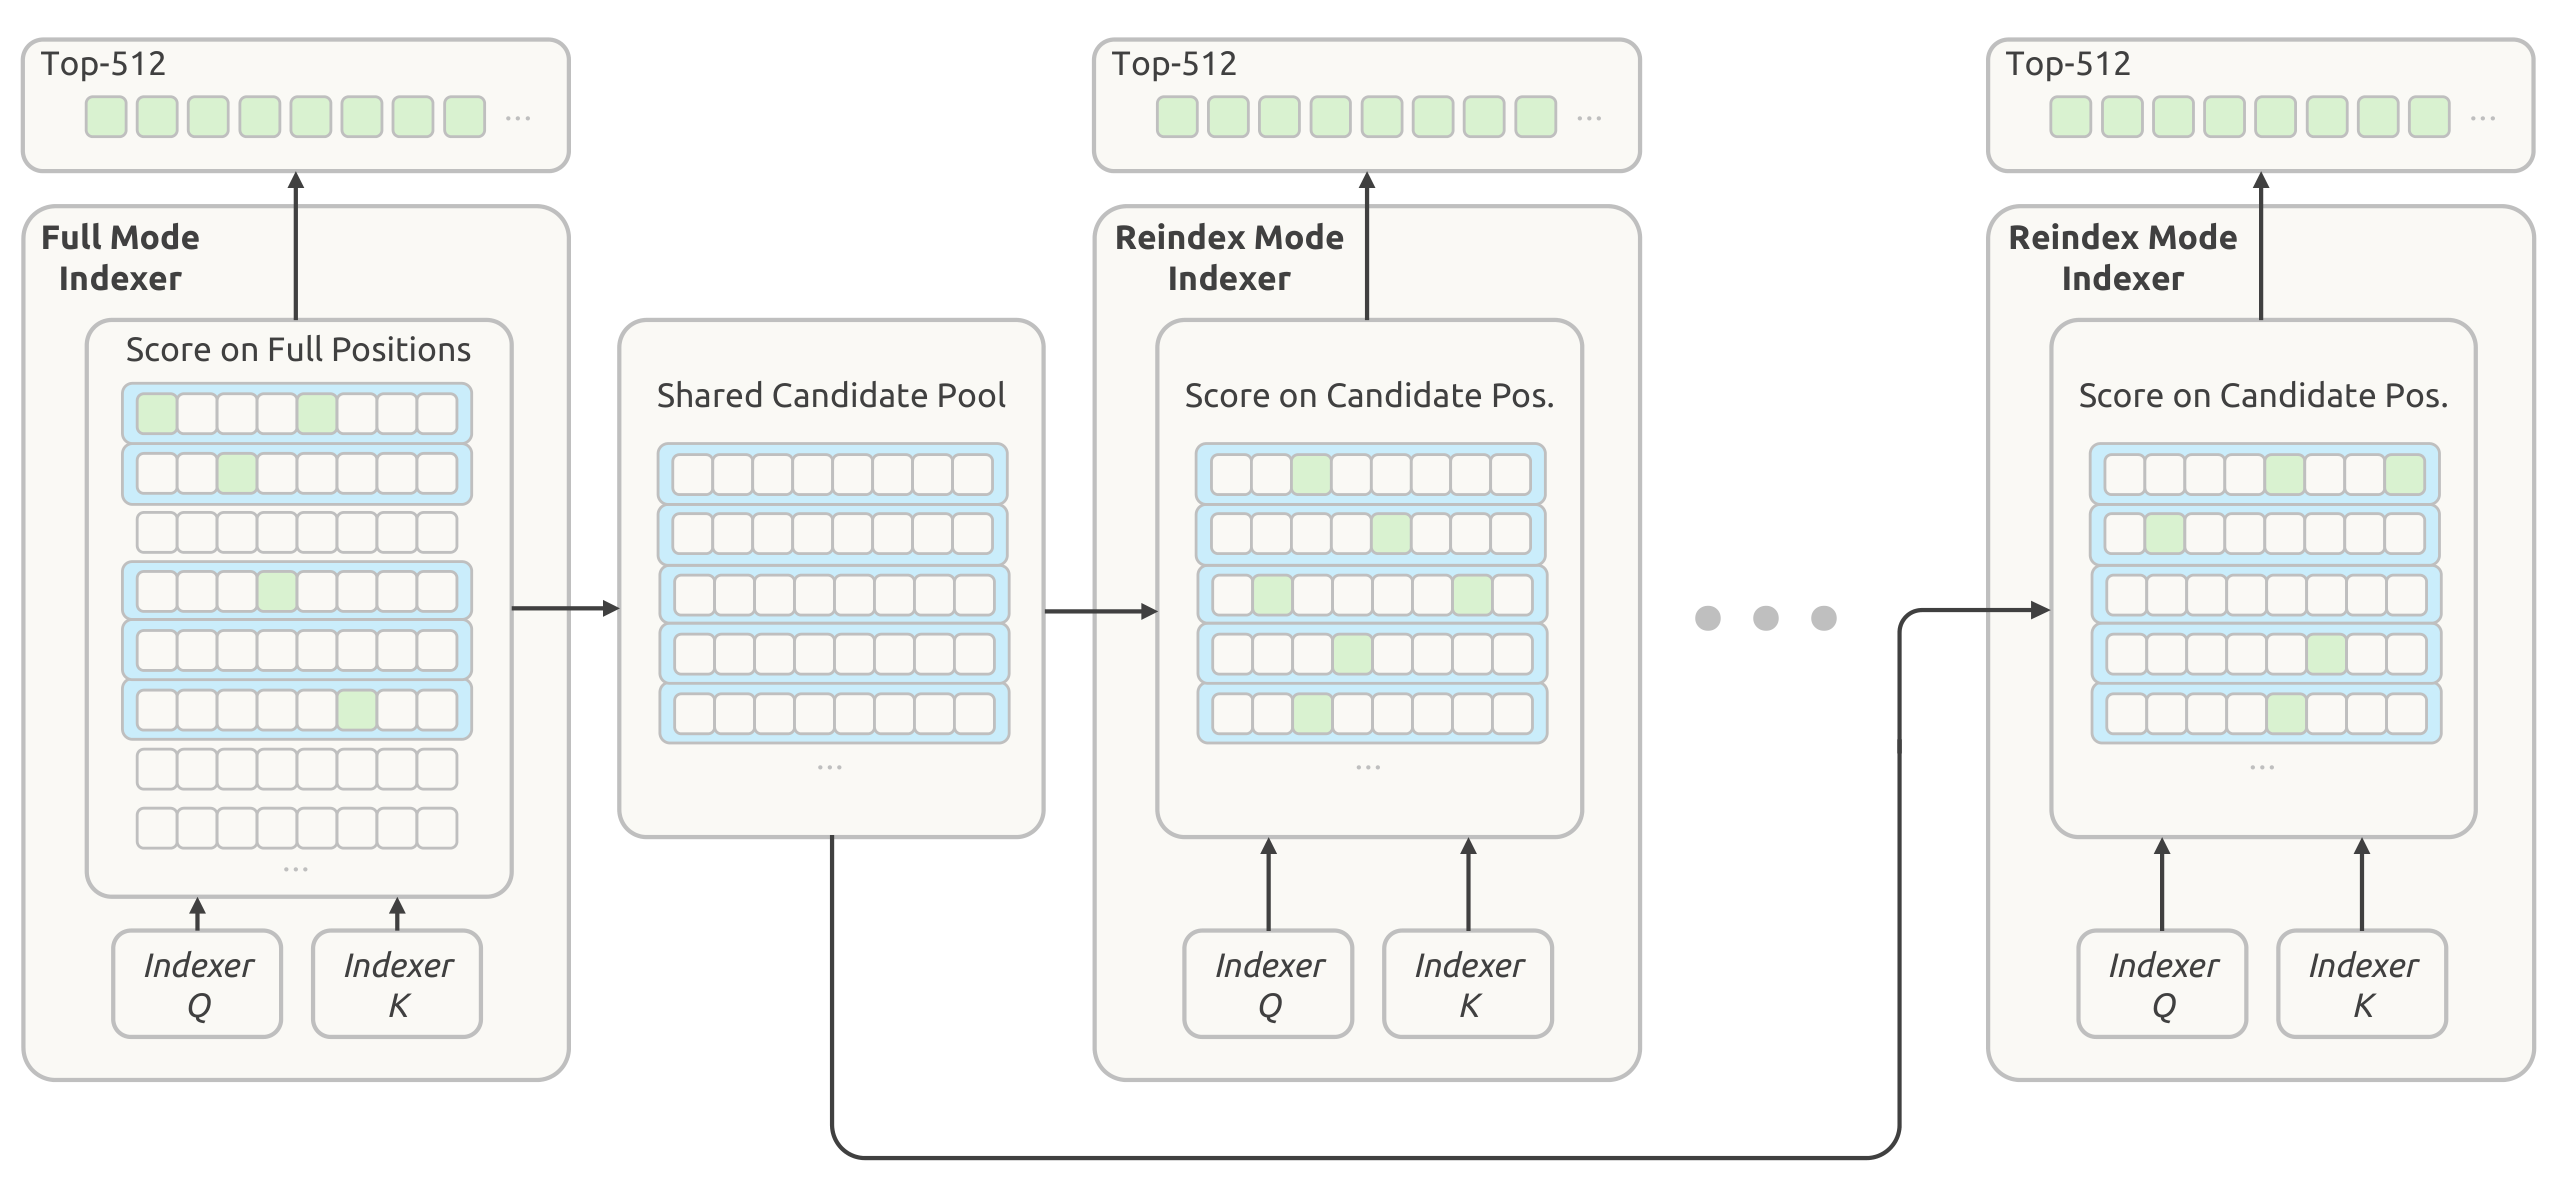
\includegraphics[width=\linewidth]{images_hi/fig05}
\caption{层次化稀疏索引器。每个方块代表一个位置；绿色方块标记被选中的索引，蓝色矩形标记基于其最大索引器得分而选中的块。解码器的第一个 CSA2 层在 Full 模式下选择自己的 Top-512 索引，并从所选块为后续层构建一个共享候选池。处于 Reindex 模式的 CSA2 层随后从该池中选择自己的 Top-512 索引。}
\label{fig:5}
\end{figure}